\section{QGIS}
QGIS adalah perangkat Sistem Informasi Geografis (SIG) Open Source yang user friendly dengan lisensi di bawah GNU General Public License. QGIS merupakan proyek tidak resmi dari Open Source Geospatial Foundation (OSGeo). QGIS dapat dijalankan pada Linux, Unix, Mac OSX, Windows dan Android, serta mendukung banyak format dan fungsionalitas data vektor, raster, dan basisdata.
Quantum GIS mendukung penggunaan "GPS tools" untuk menggunggah (upload) atau mengunduh (download) data langsung ke unit GPS. Pengguna juga dapat mengkonversi format-format GPS ke format GPX atau melakukan import dan export terhadap data format GPX yang ada.
Andaikan pengguna memiliki sebuah web server yang telah terpasang fitur UMN MapServer, pengguna dapat menpublikasi map di internet untuk berbagi (sharing) dengan pengguna lainnya.


\subsection{Getting QGIS}
\begin{enumerate}
\item
Buka browser internet Anda dan ketikkan pada bagian atas jendela browser Anda dengan tulisan qgis.org. Kemudian tekan Enter.
\begin{figure}[ht]
	    \centerline{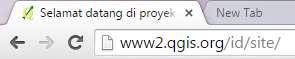
\includegraphics[width=0.50\textwidth]{figures/image1}}
	    \end{figure}

Situs resmi QGIS akan terlihat seperti ini:
\begin{figure}[ht]
	    \centerline{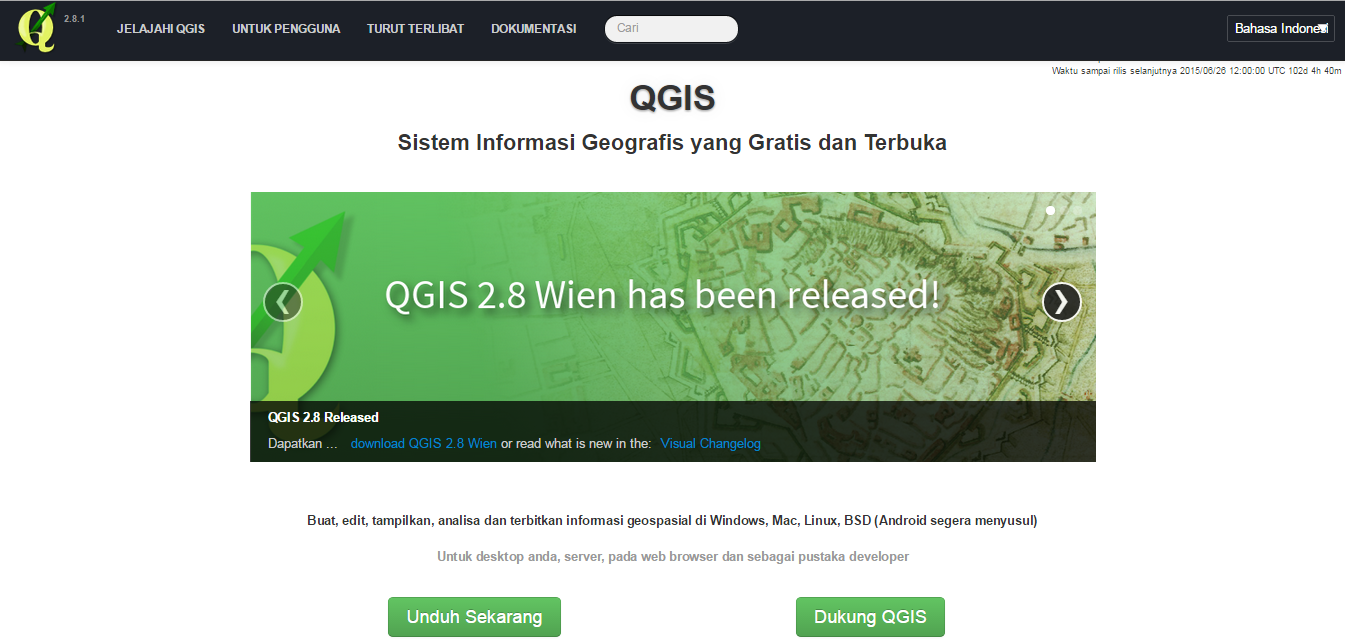
\includegraphics[width=1.00\textwidth]{figures/image2}}
	    \end{figure}
\item
Klik Unduh Sekarang
\item
Jika Anda menggunakan Windows, klik pada QGIS Standalone Installer Version 2.8 (32 bit). Nomor versi komputer Anda mungkin berbeda.
\begin{figure}[ht]
	    \centerline{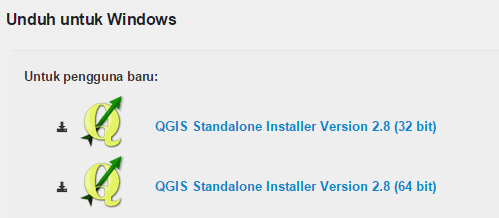
\includegraphics[width=0.50\textwidth]{figures/image3}}
	    \end{figure}
\item
Jika Anda tidak menggunakan Windows, pilih Sistem Operasi Anda dari menu yang tersedia. Ikuti intruksi instalasi.
\begin{figure}[ht]
	    \centerline{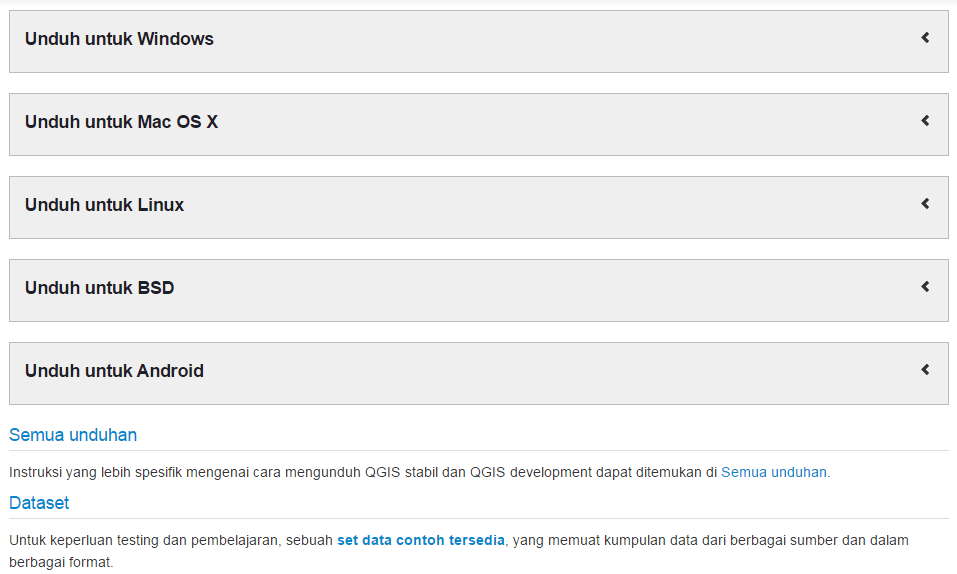
\includegraphics[width=1.00\textwidth]{figures/image4}}
	    \end{figure}
\item
Ketika file selesai didownload, jalankan dan ikuti perintah untuk menginstal QGIS.

\end{enumerate}

\subsection{Toolbar}
Pada bagian atas dari tampilan QGIS terdapat banyak sekali tool, dimana masing-masing tool tersebut masuk ke dalam beberapa kategori “toolbar”. Sebagai contoh,  file mengizinkan Anda untuk menyimpan, membuka, mencetak dan memulai proyek baru. Kita telah menggunakan salah satu alat dari toolbar file ketika kita membuka proyek baru.\ref{toolbar}.
\begin{figure}[ht]
    \centerline{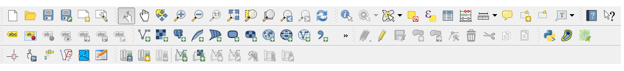
\includegraphics[width=0.25\textwidth]{figures/toolbar.png}}
    \caption{gambar toolbar yang ada pada QGis}
    \label{toolbar}
    \end{figure}

\section{Label Tool}
Label dapat ditambahkan ke dalam peta untuk menunjukkan informasi tentang objek. Suatu layer vektor dapat memiliki label yang berkaitan dengan layer tersebut. Label bergantung pada data atribut dari layer terkait.
Ada beberapa cara untuk menambahkan label pada QGIS, tetapi beberapa cara lebih baik dibandingkan yang lain. Dapat dilihat ketika membuka jendela properti dari sebuah layer, terdapat tabs yang bertuliskan "Labels". Walaupun tab ini dirancang untuk memberikan label pada peta yang dibuat, tab ini fungsinya tidak sebaik "Tool Label", yang akan dipelajari pada bagian ini. Sebelum mengakses Tool Label, harus dipastikan bahwa fitur tersebut telah diaktifkan. Berikut langkah-langkahnya :
\begin{enumerate}
\item
Pergi ke menu item View --> Toolbars
\item
Pastikan item Label telah memiliki tanda centang disebelahnya. Jika belum, klik pada item Label dan fitur tersebut akan diaktifkan.\ref
\begin{figure}[ht]
    \centerline{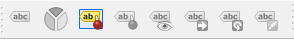
\includegraphics[width=0.25\textwidth]{figures/label.png}}
    \caption{Toolbar Label tampak seperti ini}
    \label{label}
    \end{figure}
